\section{Experimental Procedure\label{sec:TC-experimental-procedure}}
\afterpage{

\begin{figure}[H]
  \centering
  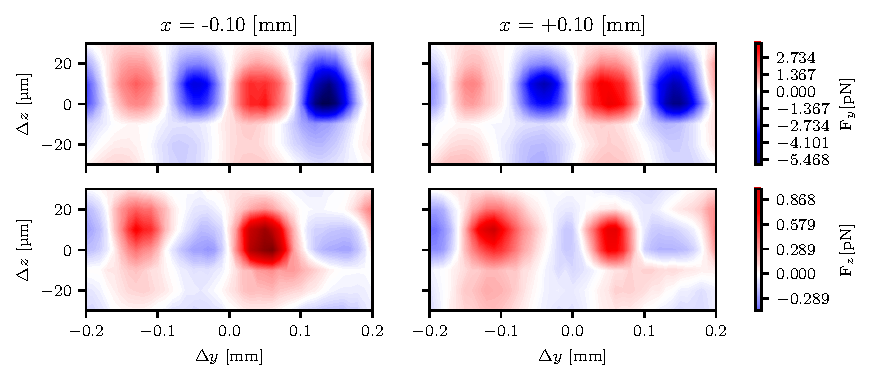
\includegraphics[width=\figWidthDouble]{\relPath/10_Figures/4um.pdf}
  % \input{10_Figures/PGF/4um_map.pgf}
  \caption{Measured steady-state acoustic forces for a \Dfour~particle with 
    $\fex=\SI{4.015}{\MHz}$ and $V_{\text{pp}} = \SI{10.7}{\volt}$. The top row 
    depicts the forces along $\ey$ and the bottom along $\ez$. The two columns 
    correspond to two different measurement $yz$-planes at $x=\SI{-0.1}{\mm}$ 
  and $x=\SI{0.1}{\mm}$, respectively.}\label{fig:TC-4um-map}
\end{figure}

\begin{figure}[H]
  \centering
  % \input{10_Figures/PGF/2um_map.pgf}
  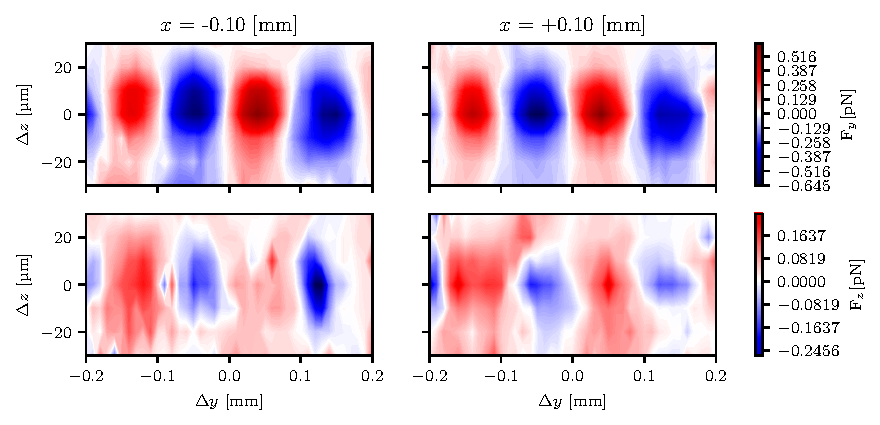
\includegraphics[width=\figWidthDouble]{\relPath/10_Figures/2um.pdf}
  \caption{Measured steady-state acoustic forces for a \Dtwo~particle with 
    $\fex=\SI{4.015}{\MHz}$ and $V_{\text{pp}} = \SI{10.7}{\volt}$. The top row 
    depicts the forces along $\ey$ and the bottom along $\ez$. The two columns 
  correspond to two different measurement $yz$-planes at $x=\SI{-0.1}{\mm}$ and 
$x=\SI{0.1}{\mm}$, respectively.}\label{fig:TC-2um-map}
\end{figure}
\clearpage
}

\subsection{Stationary Force Measurement}
In preparation for the time evolution measurement, where a spatial position of 
orthogonal AS forces and ARFs is beneficial, we characterized our device with 
two sets of stationary force measurements at a constant excitation frequency. 
For those measurements the optical trapping force is greater than the acoustic 
forces. One measurement was with a \Dtwo, and the other with a \Dfour~diameter 
particle. For changing the particle size we needed to empty and refill the 
device.  We kept the ambient conditions and experiment settings between the two 
measurements as constant as possible. For the measurements with the 
\Dtwo~particle the ambient temperature was \SI{24.49}{\celsius} in average with 
a standard deviation of \SI{0.10}{\celsius} and for the measurement with the 
\Dfour~particle the average temperature was \SI{24.78}{\celsius} with a 
standard deviation of \SI{0.25}{\celsius} ensuring the same experimental 
conditions for both measurements. More details regarding the protocol of those 
measurements can be found in \cite{Lamprecht2016} by 
\citeauthor{Lamprecht2016}.

We defined two $yz$ measurement planes, with $x_{1} = \SI{-0.1}{\mm}$ and 
$x_{2} = \SI{0.1}{\mm}$, respectively. In each plane we defined a grid in 
$y_{i}\in\{-0.20,0.19,\dots,0.20\}\,\si{\mm}$ and 
$z_{j}\in\{-30,-20,\dots,30\}\,\si{\um}$. At each point $(y_{i}, z_{j})$ we 
measured the forces in all three dimensions 5 times for \SI{3}{\second} each.  
Our excitation frequency was set to $\fex = \SI{4.015}{\MHz}$ and the applied 
voltage was $U_{\text{pp}} = \SI{10.7}{\volt}$. We choose $\fex$ based on a 
frequency sweep and the corresponding maximal forces in this sweep. With the 
chosen $\fex$ and the fluid speed of sound $\cfl \approx 
\SI{1500}{\meter\per\second}$, we obtain the theoretical acoustic wavelength of 
$\lap = \sfrac{\cfl}{\fex} \approx \SI{375}{\um}$. Hence, with the frequency 
$\fex$ and a channel width of $W = \SI{3}{\mm}$, 16 pressure nodal lines are 
present. For each spatial position we averaged the forces over the 
\SI{3}{\second} timespan and also over the 5 repetitions.

\Cref{fig:TC-4um-map,fig:TC-2um-map} visualize stationary force measurement 
results as contour plots for the two particle sizes. In addition, 
\Cref{fig:TC-averaged_forces_vs_dy} depicts the measured forces in $\ey$ and 
$\ez$ directions, when the data is additionally averaged over the 7 different 
heights $\Dz$. For \Cref{subfig:TC-F_y,subfig:TC-F_z}, the left vertical axis 
is the scale for the \Dfour~particle and the right vertical axis for 
\Dtwo~particles.

In \Cref{subfig:TC-F_y} the force wavelength $\laF$ is estimated to be 
\SI{180}{\um} which is in line with the theoretical wavelength $\laF = 
\sfrac{\lap}{2}$. One can also note that the shape of two force measurements is 
consistent. The ratio of the mean maximal force amplitudes $\frac{1.25}{0.17} = 
7.13$ is about the same as the ratio of the cubed diameter
\begin{equation}
  {\left( \frac{\Dfour}{\Dtwo} \right)}^{3} \approx 2.13^{3} \approx 9.68
 \label{eq:TC-ARF-AS-scaling}
\end{equation}
Based on the theoretical scaling laws we conclude that the forces in the $\ey$ 
direction are ARF dominant.


In \Cref{subfig:TC-F_z} one can see the measured forces in $\ez$ for both particle 
sizes and both measurement $yz$ planes. As for the forces in $\ey$ direction, 
in \Cref{subfig:TC-F_y}, the forces in $\ez$ direction are averaged over all 
$\Dz$. The force magnitude for both sizes is smaller than in $\ey$ direction 
for both particle sizes. The shapes, however, are similar but not as consistent 
as in \Cref{subfig:TC-F_y}. The ratio of the mean maximal force amplitudes 
$\frac{0.25}{0.08} \approx 3.1$ is about the same as the ratio of the two 
diameters, which suggests that in the $\ez$ direction the forces on the 
particle are AS dominated (see \Cref{eq:TC-ARF-AS-scaling}).

\begin{figure}[H]
  \centering
  \begin{subfigure}{\figWidth}
    \centering
    \caption{$F_{y}$ [\si{\pico\newton}]}\label{subfig:TC-F_y}
    % \tikzsetnextfilename{avgF_y_vs_dy}
\begin{tikzpicture}
  \begin{axis}[%
      scale only axis,
      width = 60mm,
      height = 5cm,
      axis y line*=left,
      legend style={
        fill=blue!10!white,
        font=\tiny,
        at={(0.03,0.05)},
        anchor=south west},
      xlabel = {$\Dy$ [\si{\mm}]}]

    \fill[fill=black!15!white] ({axis cs:-0.06,-2}|-{rel axis cs:0,0}) 
    rectangle ({axis cs:-0.03,2}|-{rel axis cs:0,1});

    \addlegendimage{empty legend}
    \addlegendentry{\hspace{-.6cm}\textbf{$\Rfour$}}

    \addplot[thick, blue] table[x=dy, y=F4_y1] 
    {\relPath/10_Figures/TikZ/averaged_yz_Forces.dat};
    \addlegendentry{$x_{1}$};

    \addplot[thick, blue, dashed] table[x=dy, y=F4_y2] 
    {\relPath/10_Figures/TikZ/averaged_yz_Forces.dat};
    \addlegendentry{$x_{2}$};


    \draw[|<->|] ({axis cs:-0.135,0}|-{rel axis cs:0,0.95}) -- ({axis 
    cs:0.05,0}|-{rel axis cs:0,0.95}) node[midway,below] 
    {$\sfrac{\lap}{2}=\laF$};


  \end{axis}
  \pgfplotsset{every axis y label/.append style={rotate=180,yshift=86mm}}
  \begin{axis}[%
      scale only axis,
      width = 60mm,
      height = 5cm,
      legend style={
        fill=lightgray,
        font=\tiny,
        at={(0.97,0.95)},
        anchor=north east},
      axis x line=none,
    axis y line*=right]

    \addlegendimage{empty legend}
    \addlegendentry{\hspace{-.6cm}\textbf{$\Rtwo$}}

    \addplot[thick, dotted] table[x=dy, y=F2_y1] 
    {\relPath/10_Figures/TikZ/averaged_yz_Forces.dat};
    \addlegendentry{$x_{1}$};

    \addplot[thick,loosely dashed] table[x=dy, y=F2_y2] 
    {\relPath/10_Figures/TikZ/averaged_yz_Forces.dat};
    \addlegendentry{$x_{2}$};

  \end{axis}
\end{tikzpicture}

    % \includegraphics[width=\subfigWidth]{Plots/cache/avgF_y_vs_dy.eps}
    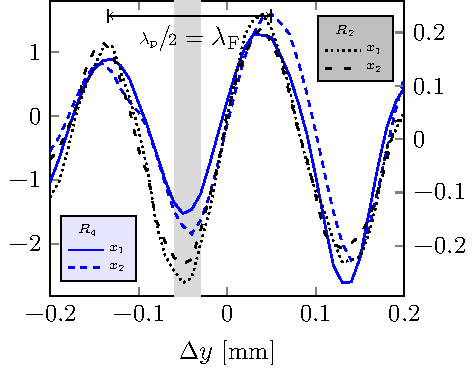
\includegraphics[]{Plots/cache/avgF_y_vs_dy.pdf}
  \end{subfigure}%
  \begin{subfigure}{\figWidth}
    \centering
    % \tikzsetnextfilename{avgF_z_vs_dy}
\begin{tikzpicture}
  \begin{axis}[%
      scale only axis,
      width = 60mm,
      height = 5cm,
      axis y line*=left,
      legend style={
        fill=blue!10!white,
        font=\tiny,
        at={(0.03,0.05)},
        anchor=south west},
      xlabel = {$\Dy$ [\si{\mm}]}]

    \fill[fill=black!15!white] ({axis cs:-0.06,-2}|-{rel axis cs:0,0}) 
    rectangle ({axis cs:-0.03,2}|-{rel axis cs:0,1});

    \addlegendimage{empty legend}
    \addlegendentry{\hspace{-.6cm}\textbf{$\Rfour$}}

    \addplot[thick,blue] table[x=dy, y=F4_z1] 
    {\relPath/10_Figures/TikZ/averaged_yz_Forces.dat};
    \addlegendentry{$x_{1}$};

    \addplot[thick, blue, dashed] table[x=dy, y=F4_z2] 
    {\relPath/10_Figures/TikZ/averaged_yz_Forces.dat};
    \addlegendentry{$x_{2}$};

  \end{axis}
  \pgfplotsset{every axis y label/.append style={rotate=180,yshift=86mm}}
  \begin{axis}[%
      scale only axis,
      width = 60mm,
      height = 5cm,
    axis y line*=right,
      yticklabel style={
        /pgf/number format/fixed,
        /pgf/number format/precision=2
      },
      legend style={
        fill=lightgray,
        font=\tiny,
        at={(0.97,0.95)},
        anchor=north east},
      axis x line=none]

    \addlegendimage{empty legend}
    \addlegendentry{\hspace{-.6cm}\textbf{$\Rtwo$}}

    \addplot[thick, dotted] table[x=dy, y=F2_z1] 
    {\relPath/10_Figures/TikZ/averaged_yz_Forces.dat};
    \addlegendentry{$x_{1}$};

    \addplot[thick,loosely dashed] table[x=dy, y=F2_z2] 
    {\relPath/10_Figures/TikZ/averaged_yz_Forces.dat};
    \addlegendentry{$x_{2}$};

  \end{axis}
\end{tikzpicture}

    % \includegraphics[width=\subfigWidth]{Plots/cache/avgF_z_vs_dy.eps}
    \caption{$F_{z}$ [\si{\pico\newton}]}\label{subfig:TC-F_z}
    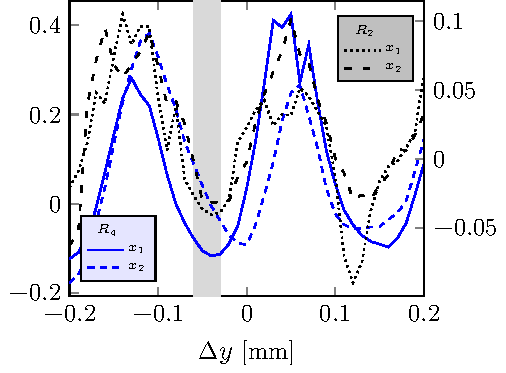
\includegraphics[]{Plots/cache/avgF_z_vs_dy.pdf}
  \end{subfigure}%
  \caption{Measured steady-state acoustic forces when averaged over the cavity 
    height. All values are in \si{\pico\newton}. For each plot the left 
    $y$-axis is the measured force on the \Dfour~($D_{4}$) particle and the 
    right one for the \Dtwo~($D_{2}$) particle, respectively.
    The gray shaded area corresponds to the positions where the time evolution 
  is measured.}\label{fig:TC-averaged_forces_vs_dy}
\end{figure}

\subsection{Measurement Protocol for Time Evolution}

Based on a set of proof-of-concept experiments (data not shown here) and the 
information from numerical simulations that the AS field in a \emph{real} 
device can substantially differ from the AS field of fluid cavity-only 
structure, we selected $x = 0$, $y_{i} \in 
\{-0.15,-0.14,\dots,0.10\}\,\si{\mm}$, and $z_{j} \in \{-10,0,10\}\,\si{\um}$. 
This choice means, that we measure at the same $y_{i}$ and $z_{j}$ as for the 
stationary force measurement. We have the same excitation frequency ($\fex = 
\SI{4.015}{\MHz}$) as in the stationary force measurements from before. However 
we set the excitation amplitude slightly higher to $U_{\text{pp}} = 
\SI{11.7}{\volt}$ in order to increase the signal to noise ratio (SNR).

We control the whole measuring routine with a self-written Python program. 
Before each measurement, the offset of the QPDs is checked and, if needed, 
adjusted. First we measure without US and then we measure with US on. We repeat 
this procedure 50 times before moving to the next location.

For the time evolution measurement, we acquire with a sampling rate of $\fs 
=\SI{1.25}{\MHz}$ ($\Dt = \SI{0.8}{\us}$) for \SI{125}{\ms} the three QPD 
signals, the signal for the shutter, and the DC signal for the laser as soon as 
the shutter starts opening ($t = \SI{-25}{\ms}$ in \Cref{fig:TC-daq-sync}). 
Between $t =\SI{0}{\ms}$ and $t = \SI{30}{\ms}$ the shutter is completely open 
and the US is switched on. Extending the measurement time further has no 
benefit because the particle will be outside the linear regimes of the QPDs and 
might move too far from the OT trapping region such that it cannot be 
recaptured after the laser changes to its high power state again.

We repeat 50 times per position because the particle starts sedimenting 
as soon as the laser power drops to the lower value. During this movement the 
particle still undergoes Brownian motion. Hence, the trajectory is not straight 
along the $\ez$ direction. With 50 datasets, we can average this random 
movement out.

Taking the approximation of \cref{eq:TC-mod-free-fall} into account, a \Dtwo~large 
\SiO~sphere sedimenting in water reaches its terminal velocity 
almost instantaneously, because the inertia term is small; additionally, the 
sphere travels about $0.12\,\Rtwo$ in \SI{55}{\ms}. Therefore, after 
\SI{25}{\ms} the particle is still in the linear regime of the QPDz. The static 
gravitational force ($\tilde{m}g$) with the added buoyancy of water is less 
than \SI{40}{\femto\newton} for the \Dtwo~particle. This is more than 6 times 
smaller than the maximal measured force in $\ez$ direction. Therefore, we 
assume in areas of maximal forces along $\ez$ that the driving force of this 
movement is either the acoustic field or $\FAS$. With an ideal sedimentation in 
the first \SI{25}{\ms} along $\ez$, the laser spot on QPDxy does not change at 
all during the sedimentation.

\subsection{Data Processing}

The acquired data is postprocessed with Python. We look at discrete points 
every $t_{k} = k\cdot\SI{0.1}{\ms}$ with $k\in \mathbb{N}$. In addition, we use 
a moving average for the data at $t_{k}$ with a centered window size of 101 
data points, corresponding to a timespan of \SI{80}{\us}. Next, we subtract the 
data series without US from the series with US to obtain the delta voltage 
$\DV_{m}$, with $m$ being $y$ or $z$. This quantity allows us to further reduce 
unwanted noise. This step serves also as data quality check because all 
measurements have the same protocol until $t=\SI{0}{\ms}$. Hence, the delta 
voltage $\DV_{m}$ must be \emph{zero} for $t\leq\SI{0}{\ms}$. Then, we average 
$\DV_{m}$ over the 50 repetitions per spatial position $y_{i}, z_{j}$. As last 
step for the time evolution plots, we normalize the data by the $\max\left( 
\left\vert \DV_{m}(t)\right\vert \right)$ for $\SI{10}{\ms} < t < 
\SI{30}{\ms}$.
